\RequirePackage{fixltx2e}
\documentclass[
  captions=tableheading,  % Tabellenüberschriften
  titlepage=false, % Titelseite ist Deckblatt
  twocolumn,
  headings=small,
]{scrartcl}

\usepackage[aux]{rerunfilecheck}

\usepackage{polyglossia}
\setmainlanguage{german}

\usepackage{microtype}

\usepackage{fontspec}
\defaultfontfeatures{Ligatures=TeX}

\usepackage[autostyle]{csquotes}

\usepackage[
  locale=DE,                   % deutsche Einstellungen
  per-mode=symbol-or-fraction, % m/s im Text, sonst Brüche
]{siunitx}

\usepackage{xfrac}

\usepackage[section, below]{placeins}
\usepackage[
  labelfont=bf,        % Tabelle x: Abbildung y: ist jetzt fett
  font=small,          % Schrift etwas kleiner als Dokument
  format=plain,
]{caption}
\usepackage{subcaption}
\usepackage{graphicx}
\usepackage{grffile}
\usepackage{wrapfig}

\usepackage{scrhack}
\usepackage{float}
\floatplacement{figure}{htbp}
\floatplacement{table}{htbp}

\usepackage{booktabs}

\usepackage[
  unicode,
  pdfusetitle,    % Titel, Autoren und Datum als PDF-Attribute
  pdfcreator={},  % PDF-Attribute säubern
  pdfproducer={}, % "
]{hyperref}
\usepackage{bookmark}
\usepackage[shortcuts]{extdash}

\title{Projekt-Dokumentation}
\subtitle{Pep et. Al. Sommerakademie}
\date{24. -- 31. August 2014}

\author{Johannes Bieker \and Henning Moldenhauer \and Max Nöthe}

\begin{document}
\maketitle
\section*{3D-Filme}
\begin{center}
  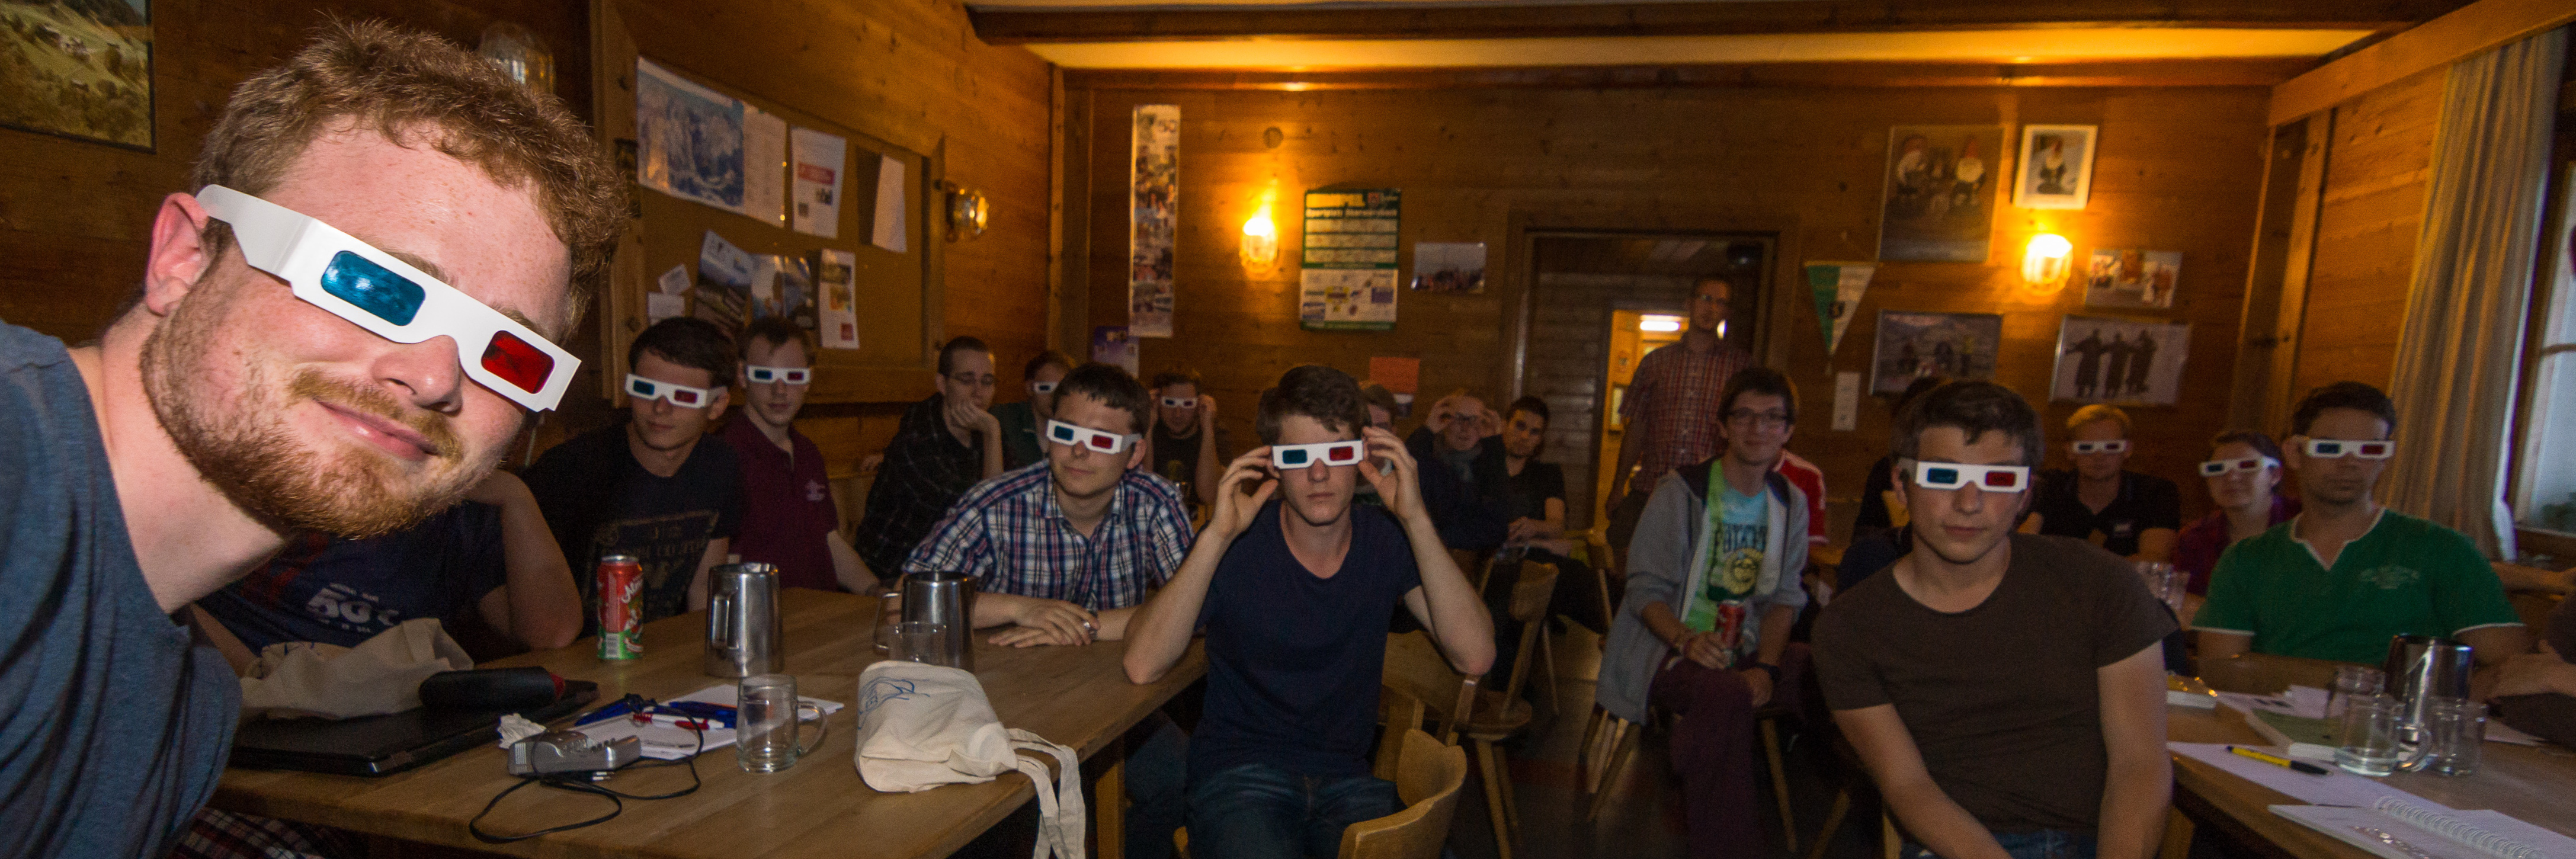
\includegraphics[width=\linewidth]{images/3dfilme_panorama.JPG}
\end{center}
Im Rahmen der diesjährigen Sommerakademie gab es die Idee 3D-Filme zu erstellen.
Um einen dreidimensionalen Effekt zu erhalten, muss das selbe Objekt aus zwei verschiedenen Winkeln betrachtet werden.
Damit der Effekt möglichst realistisch wirkt, sollte der Abstand der beiden Kameras dem Abstand menschlicher Augen entsprechen.
Es standen dazu zwei GoPros, Farbfilter und die nötige Software (StereoMovie Maker, Bino) zur Verfügung.

Die Problemstellung lag auf der Suche nach korrekten Kameraeinstellungen und notwendigem Abstand zwischen Objekt und Kamera.

Es zeigte sich, dass zwingend auf baugleiche Kameras zu achten ist, was bei den verwendeten GoPros nicht der Fall war.
Durch die ungleiche Bauweise wurden Farben unterschiedlich wiedergegeben, sodass Ghosting entstand.
Der Mindestabstand von Objekt zu den Kameras sollte 5 Meter betragen, da auch hier sonst wieder verstärkt Ghosting zu beobachten war.
Mit zwei baugleichen Handy-Kameras konnten erfolgreich 3D-Filme ohne Ghosting produziert werden.

\section*{Temperaturkontrolle mit Arduinos}
Ziel dieses Projektes war es eine Temperaturüberwachung des Solarofens zu realisieren.
Wichtig war dabei die korrekte Kalibration des Temperatursensors.
Zur leichteren Bedienung sollte die Temperatur mittels LCD-Display dargestellt werden.

Als Problem stellte sich heraus, dass im Solarbrenner Temperaturen größer der Lotschmelztemperatur erreicht werden können.
Temperaturen dieser Art kann der Sensor zwar messen, jedoch lösen sich dann die Kabelverbindungen ab.

Der Sensor konnte noch nicht am Brenner verwendet werden, wurde jedoch bereits bei der Temperaturkontrolle der Nebelkammer eingesetzt.

\section*{Astrofotografie-Nachführung}
Bereits auf der letzten Sommerakademie wurde damit begonnen astronomische Objekte zu fotografieren.
Um längere Belichtungszeiten zu erreichen und somit auch lichtschwächere Objekte beobachten zu können, wurde in diesem Jahr eine einfache mechanische Nachführung, genannt Barndoor, gebaut.

Als problematisch stellte sich die nicht ideale Krümmung der per Hand gebogenen Gewindestange heraus.
Eine weitere Schwierigkeit war die Ausrichtung der Drehachse der Nachführung auf den Himmelsnordpol.
Hier ließen sich durch eine optimierte Zielvorrichtung bessere Bilder aufnehmen.
Durch starke Bewölkung war die Beobachtungszeit außerdem stark eingeschränkt.

Mit der Nachführung lassen sich jedoch bereits Belichtungszeiten von 8 Minuten bei \SI{8}{\milli\meter} Brennweite erstellen.
Im letzten Jahr, ohne Nachführung, ließ sich nur eine Belichtungszeit von 15 Sekunden bei \SI{16}{\milli\meter} erreichen.

\begin{figure}
  \centering
  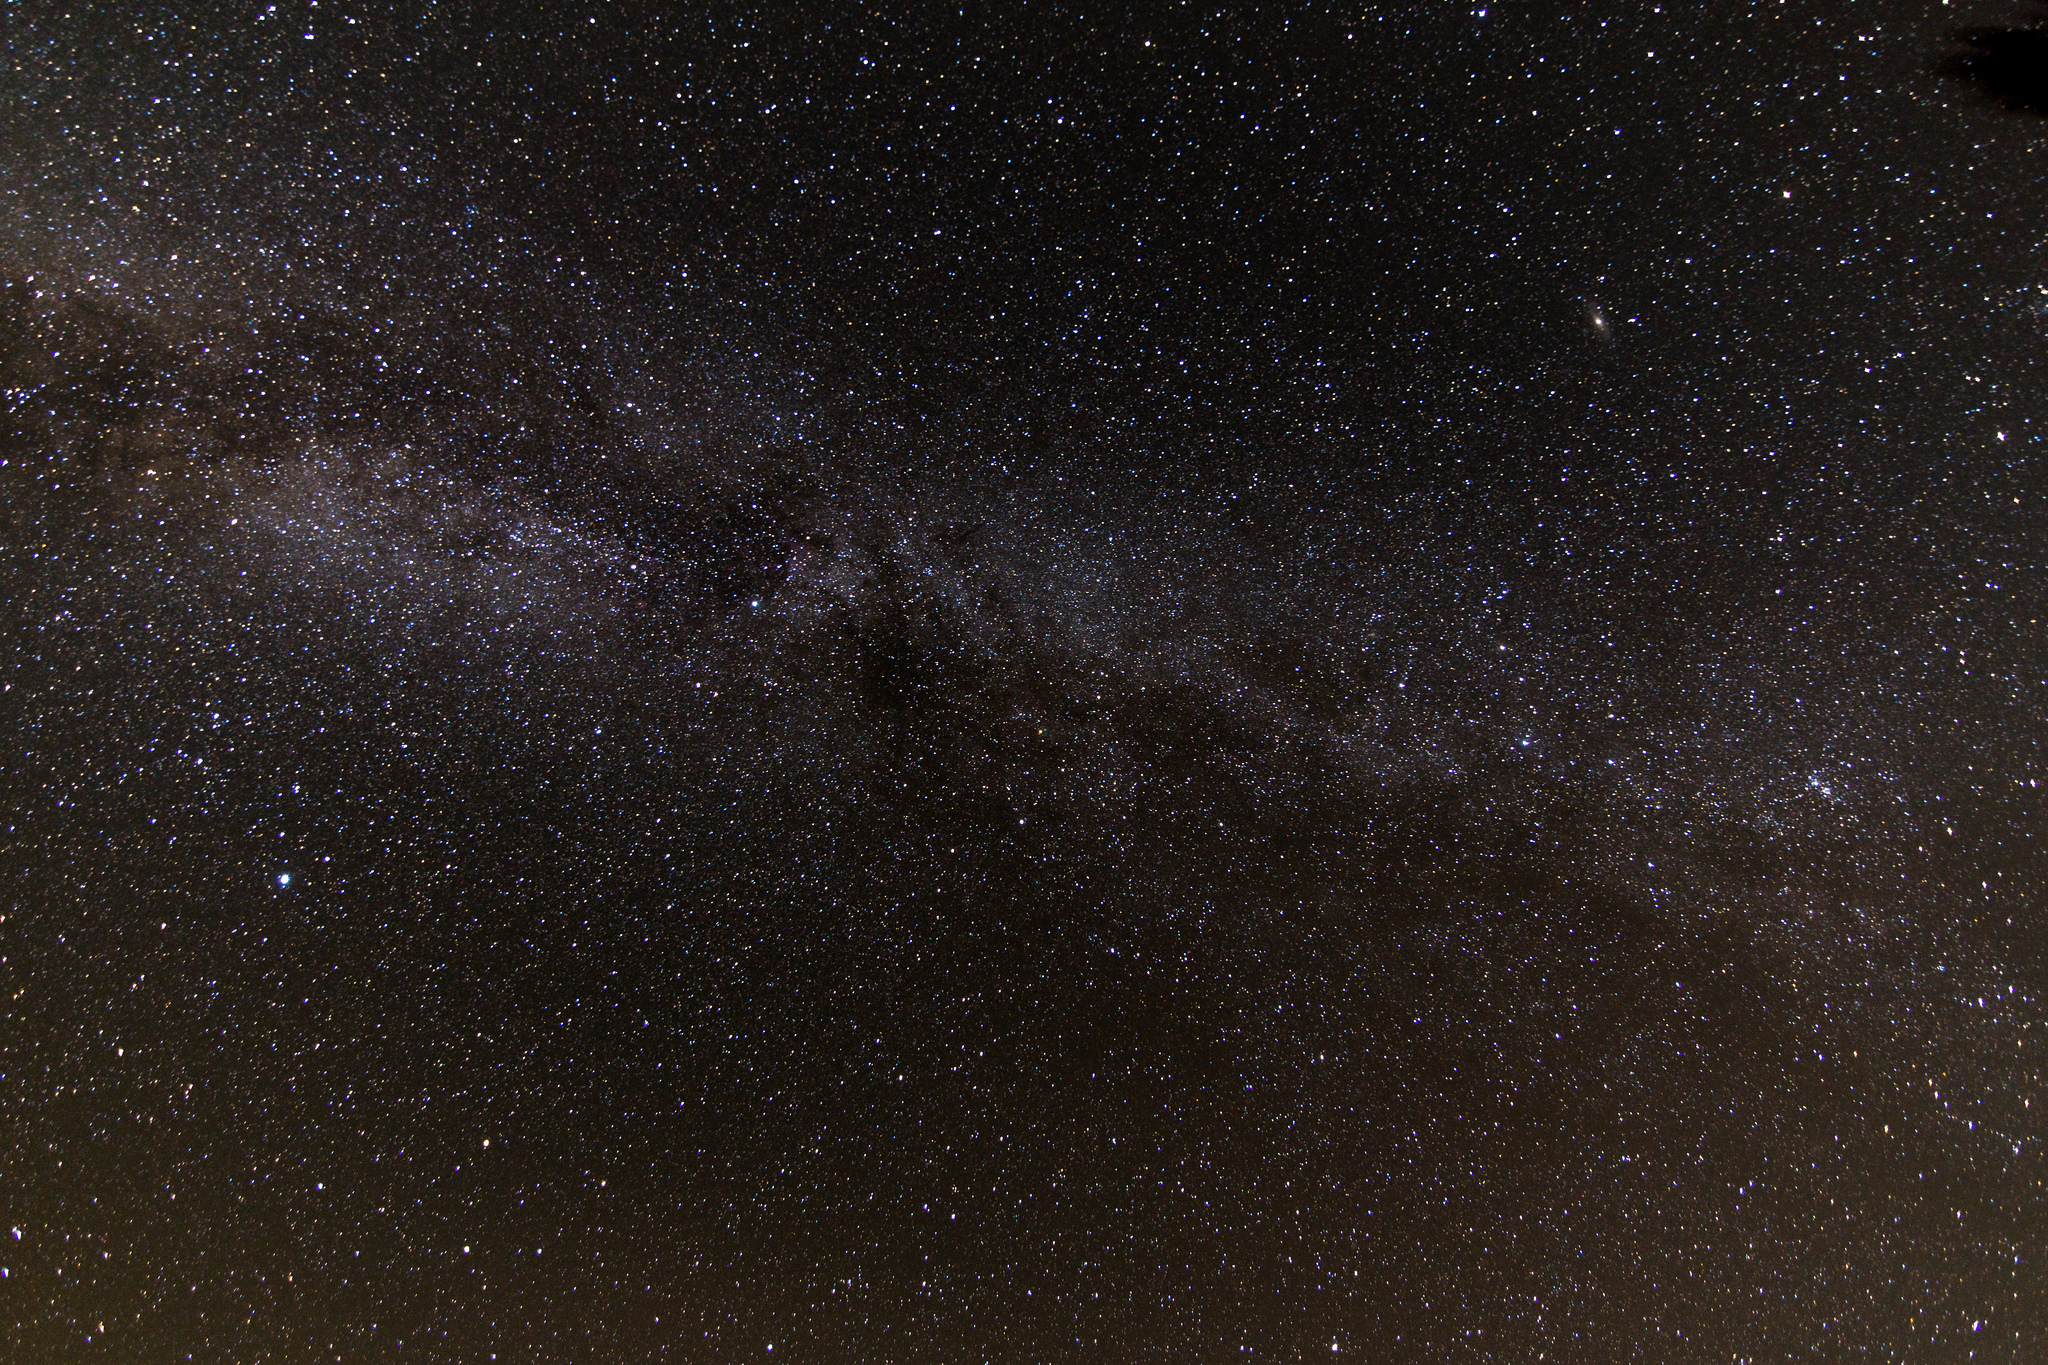
\includegraphics[width=\linewidth]{./images/milkyway.jpg}
  \caption{Aufnahme der Außenbereiche der Milchstraße, M31 ist als heller Fleck im rechten oberen Drittel zu sehen.}
\end{figure}


\section*{Nebelkammer}
\begin{center}
  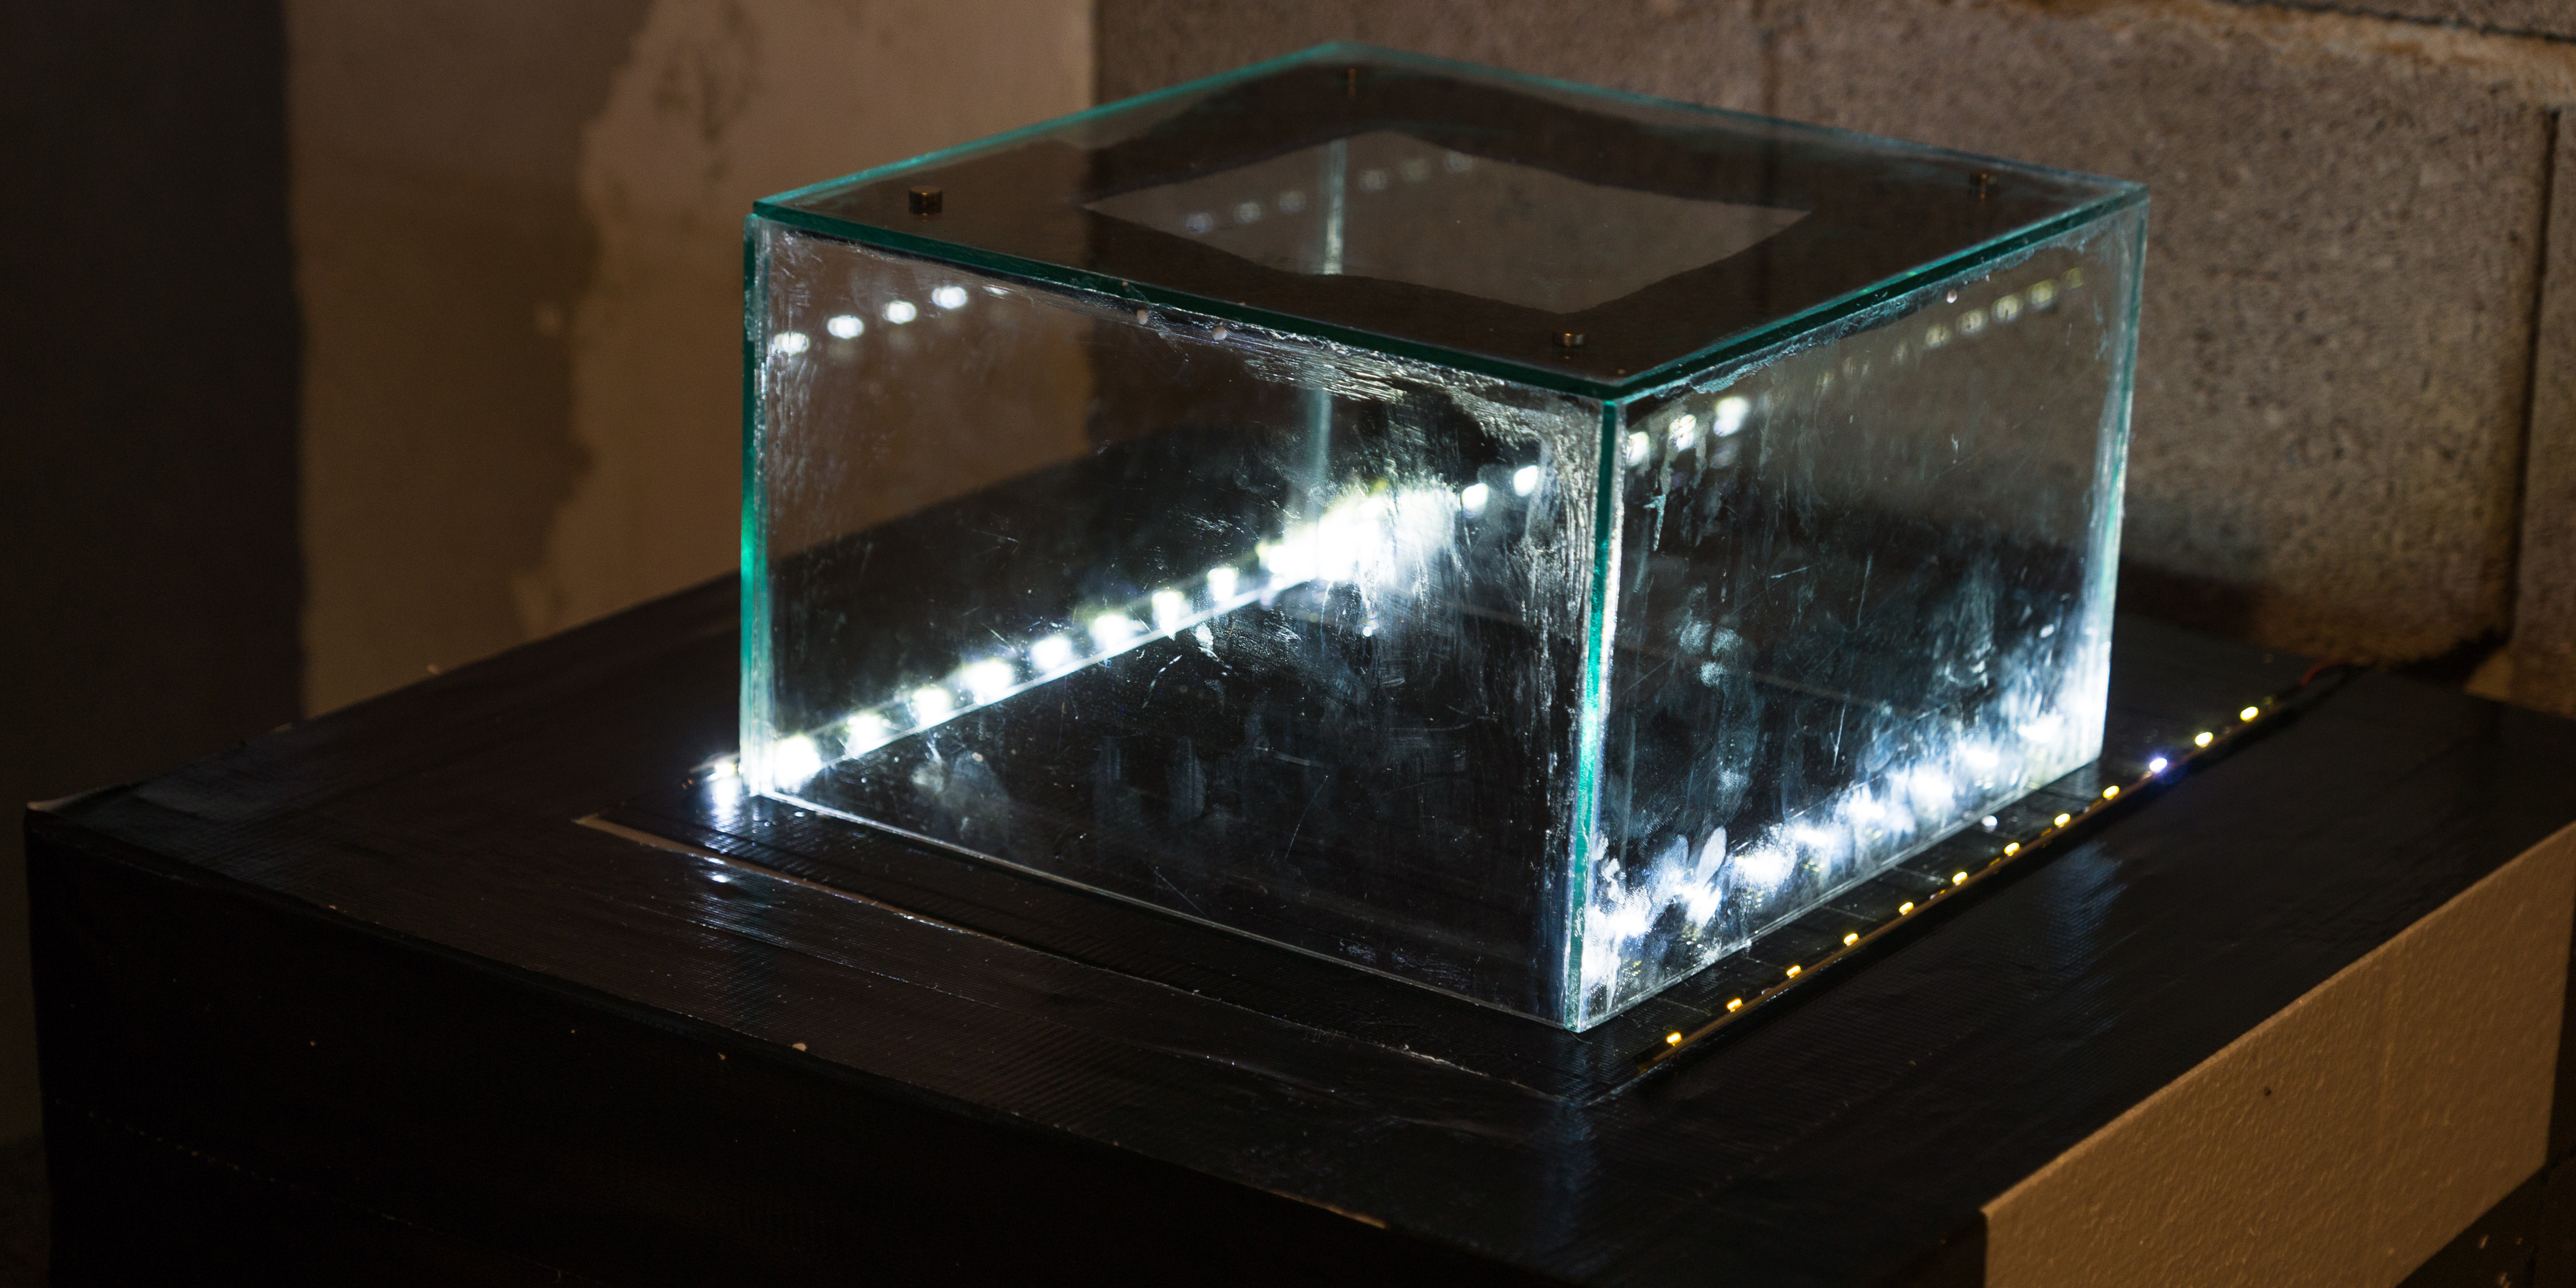
\includegraphics[width=\linewidth]{./images/nebelkammer_aufbau.JPG}
\end{center}
Der Bau einer Nebelkammer sollte ein weiteres Projekt der diesjährgen Sommerakademie darstellen.
Ziel war der Nachweis geladener Teilchen durch Beobachtung ihrer Spuren in einem Isopropanolnebel.
Damit sich ein Nebel ausbildet, wurde eine mit Trockeneis gekühlte Metallplatte am Boden eines umgekehrten Aquariums verwendet.

Optimieren ließe sich die Kammer durch eine bessere Abdichtung, sowie die Verwendung einer schwarz lackierten Metallplatte.
Statt mit Trockeneis ließe sich die Kammer auch über Peltierelemente kühlen.
Um mehr Spuren zu beobachten, könnte man eine radioaktive Quelle untersuchen.
\begin{figure}
  \centering
  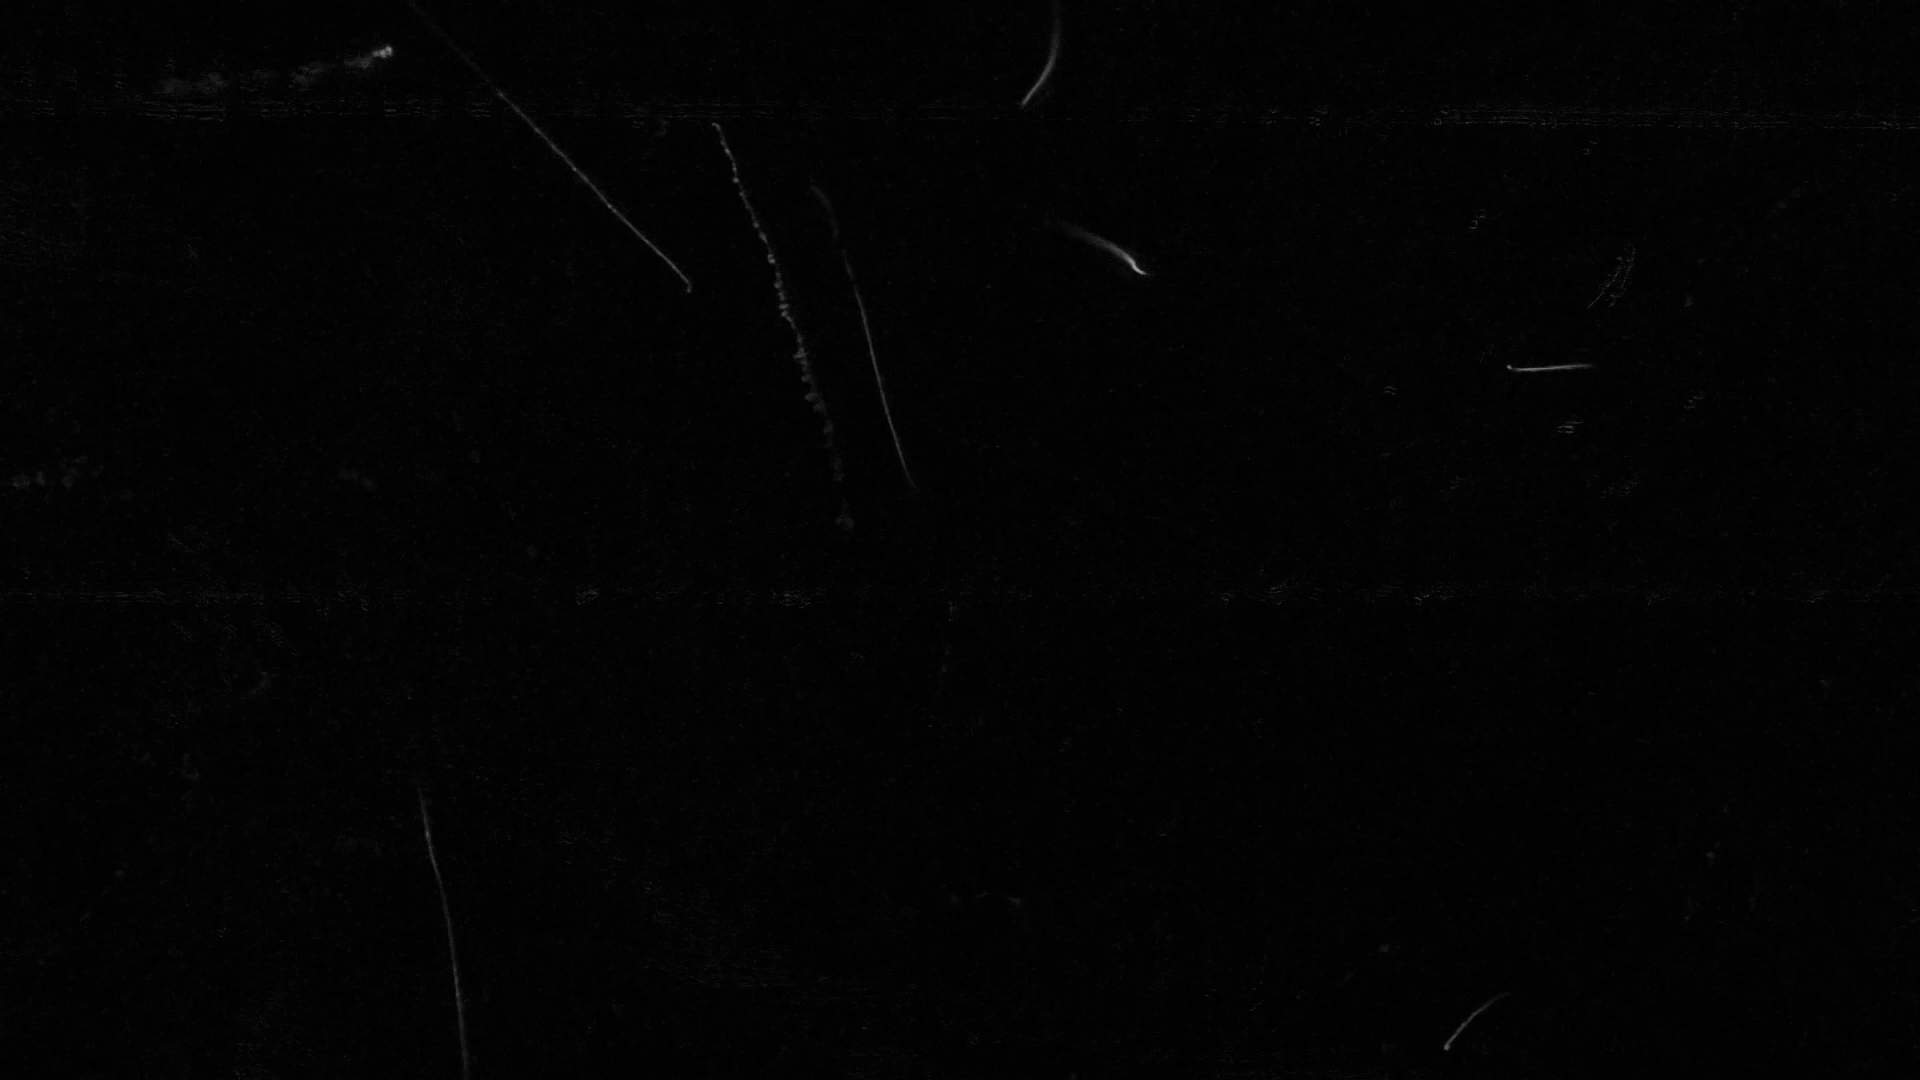
\includegraphics[width=\linewidth]{./images/nebelkammer_spuren.png}
  \caption{Kombiniation mehrerer Bilder von aufgenommen Spuren in der Nebelkammer.}
\end{figure}

\section*{Microblog}
Aus der Idee mit Hilfe eines RasPi ein mobiles drahtloses Netzwerk einzurichten, entstand schnell die Notwendigkeit einer geeigneten Kommunikationsplattform.
Das primäre Ziel der Software war die Speicherung von Text- und Bildbeiträgen von verschiedenen Nutzern, sowie die chronologische Wiedergabe dieser Beiträge.
Zusätzliche Funktionen wie das Liken oder das Verstecken von Nachrichten wurden ebenfalls implementiert.

Die Mobilität des Systems wurde unter Verwendung eines USB-Akkus bei der Wanderung auf die Mittagsspitze erfolgreich getestet.

Um die Reichweite des RasPi zu erhöhen, wurde im Ferienhaus mit einem externen Router verstärkt.

Durch den Microblog entstand eine lustige und sehenswerte Live-Dokumentation der Sommerakademie.
\begin{figure}
  \centering
  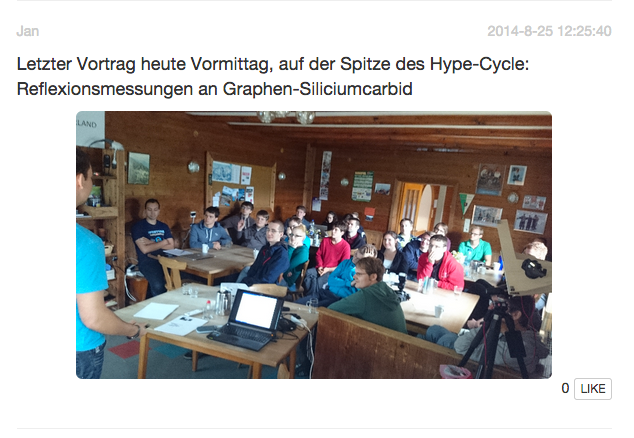
\includegraphics[width=\linewidth]{./images/microblog_screenshot.png}
  \caption{Screenshot eines Beitrags aus dem Microblog.}
\end{figure}

\section*{Wasserrakete}
\begin{wrapfigure}{l}[0.1\linewidth]{0.2\linewidth}
  \centering
  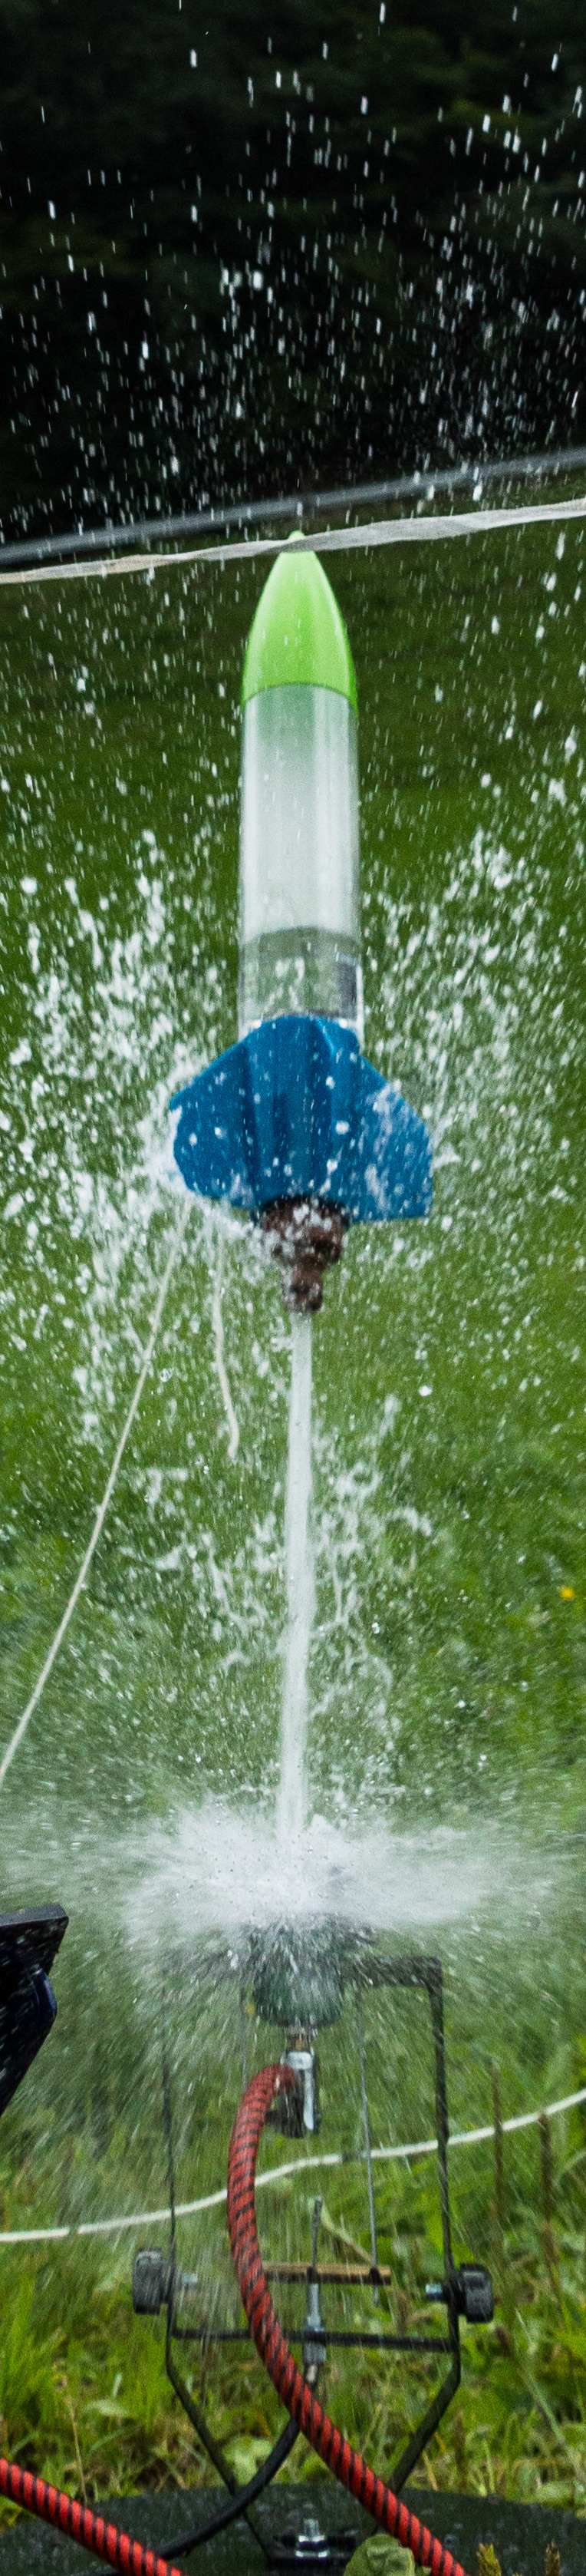
\includegraphics[width=\linewidth]{./images/wasserrakete_schmal.JPG}
\end{wrapfigure}
Dieses Projekt war eine Weiterentwicklung der Wasserrakete aus dem letzten Jahr.
Die Absicht war die Rakete höher fliegen zu lassen und damit länger in der Luft zu halten.

Es wurden zwei mögliche Optimierungen für die Rakete ausprobiert:
Zur Minderung der Fallgeschwindigkeit, damit die Rakete beim Landen nicht beschädigt wird, wurde ein Fallschirm angebracht.
Dieser verringerte die Flughöhe der Rakete jedoch sehr.
Damit die Rakete eine bessere Flugbahn beschrieb, wurde ein sich selbsständig ausfahrendes Leitwerk montiert.
Unter Verwendung des Leitwerks konnte die Rakete größere Höhen erreichen.

Probleme bereiteten die nicht druckbeständigen Klebestellen, sowie ein unkontrollierter Start bei \SI{5}{\bar} und eine nicht zuverlässige Entfaltung des Fallschirms.

\section*{Solarofen}
Auch dieses Projekt war eine Fortführung eines letztjährigen Projektes.
Es sollte ein Ofen aus einer Kiste gebaut werden.
Mittels eines Spiegels wurde Sonnenlicht durch einen Glasdeckel in diesen reflektiert, sodass sich das Innere des Ofens erwärmte.

Das Innere der Kiste wurde mit geschwärzten Aluminiumplatten ausgekleidet, damit einfallende Strahlung absorbiert wird.
Die erhoffte Temperatursteigerung blieb aus.
Für einen Langzeittest des Ofens gab es nicht ausreichend Sonnenstunden.

\section*{Solarkocher}
\begin{wrapfigure}{r}[0.1\linewidth]{0.3\linewidth}
  \centering
  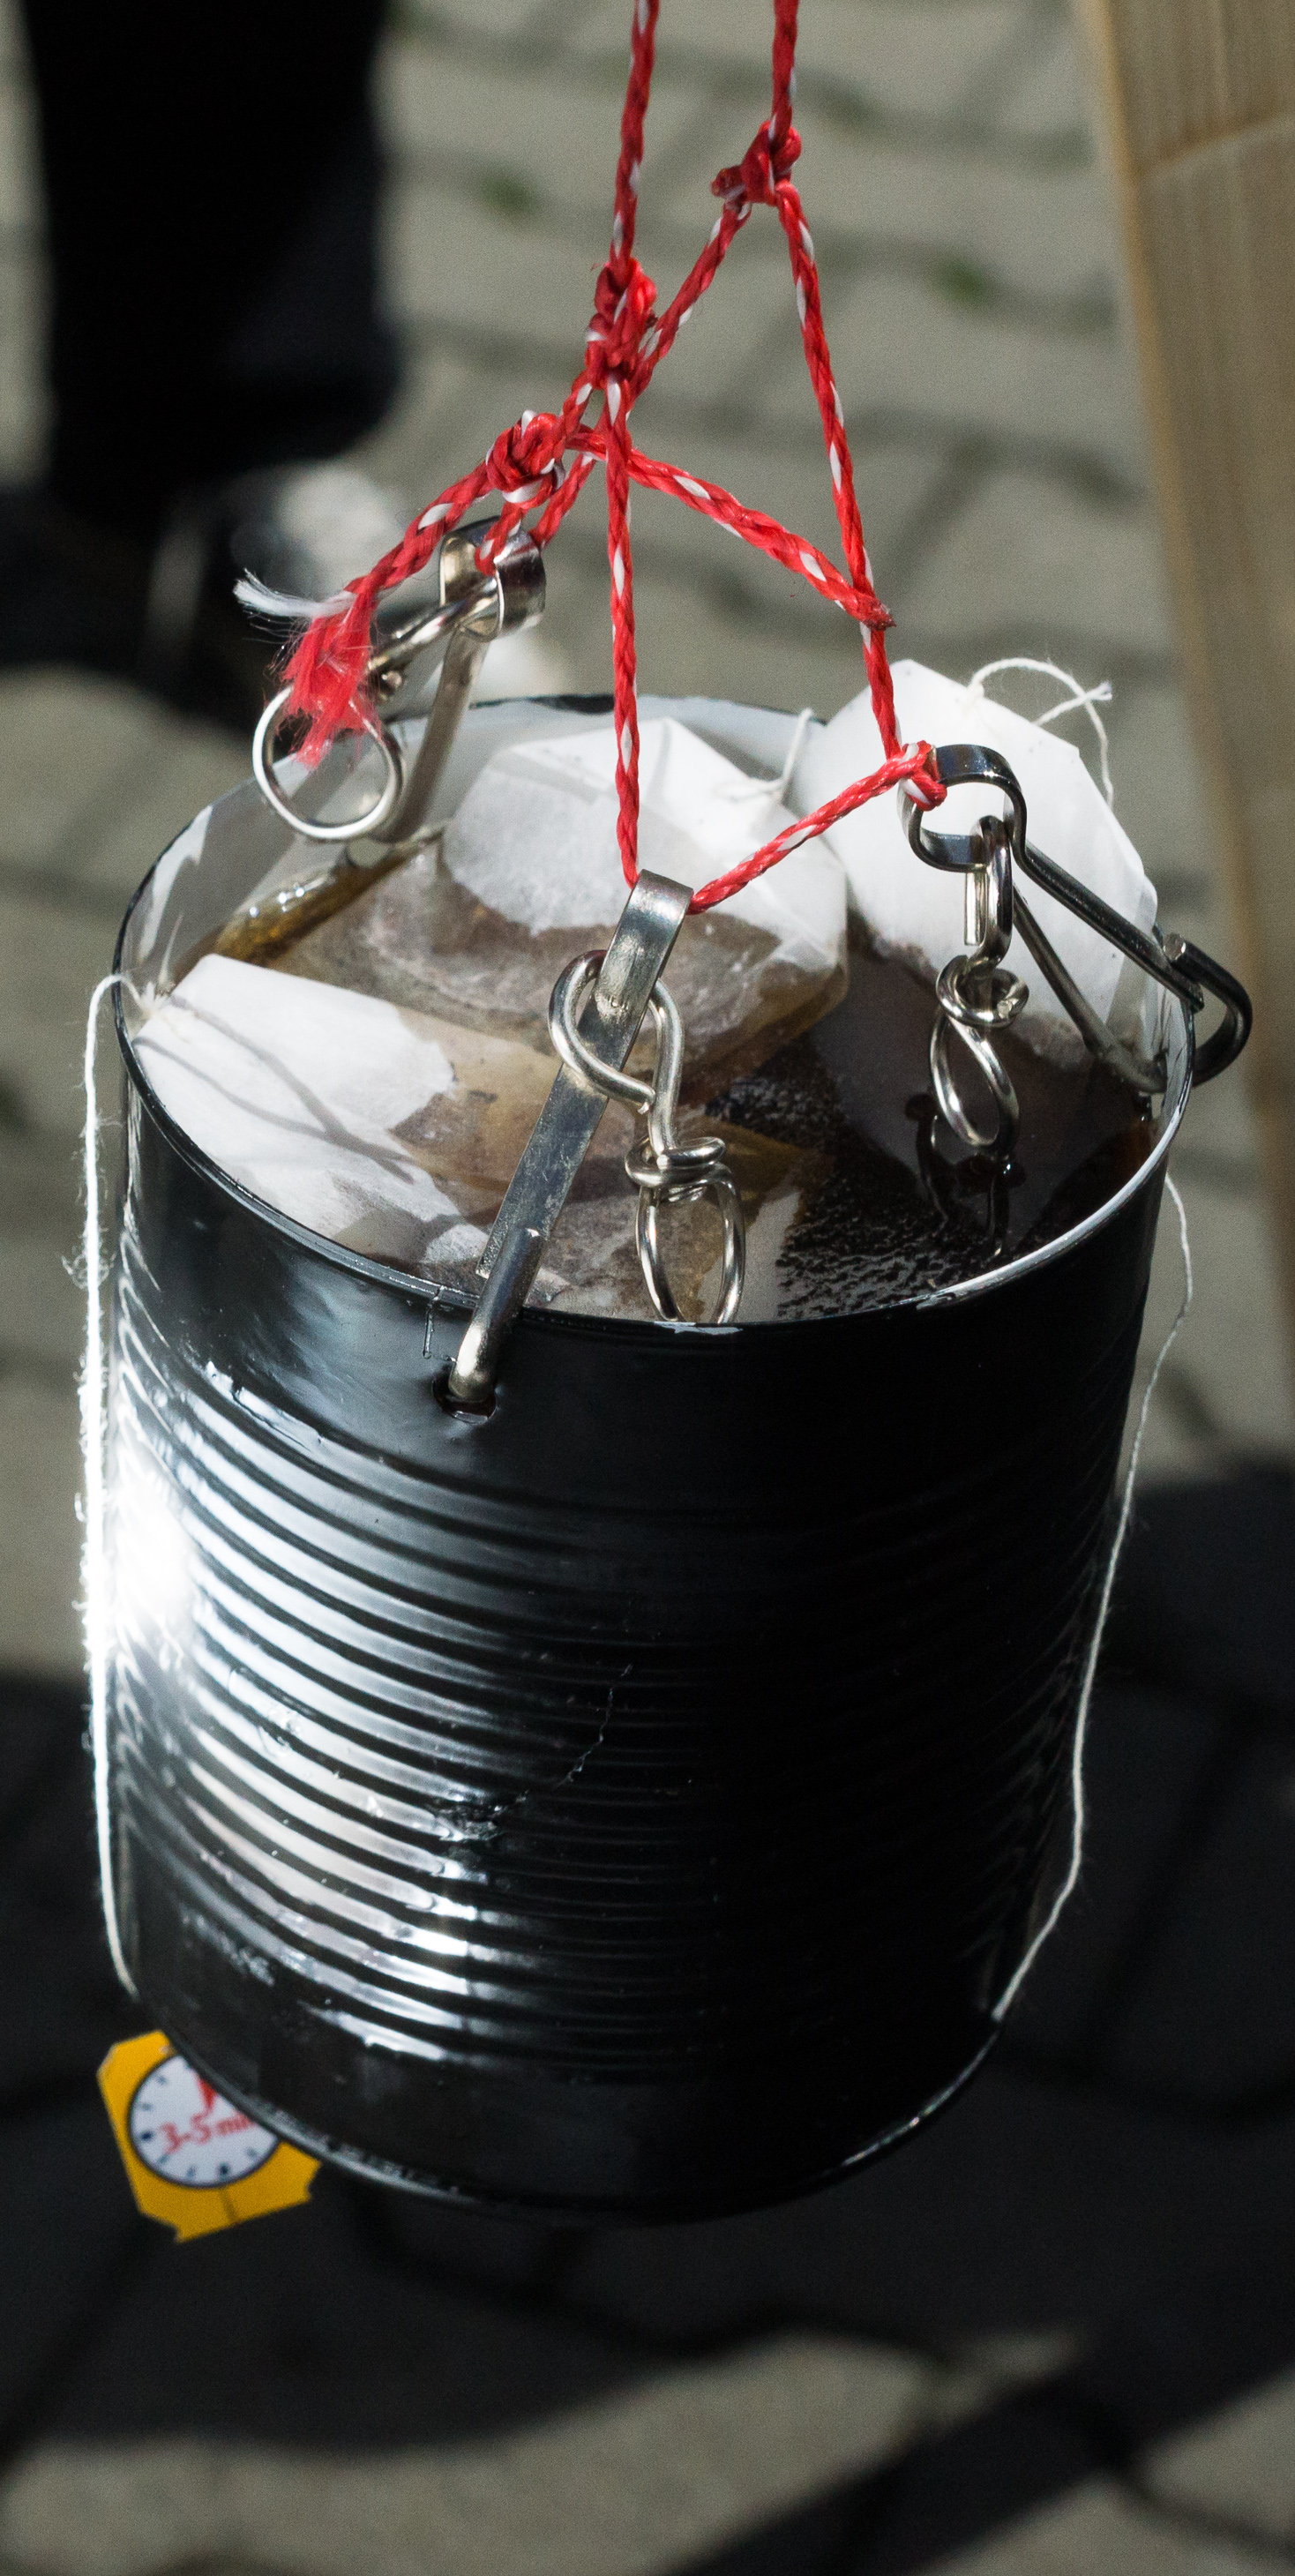
\includegraphics[width=\linewidth]{./images/solarkocher_tee.JPG}
\end{wrapfigure}
Ziel war es mittels Sonnenlicht kochen zu können.
Verwendet wurde dazu eine mit Spiegelfolie überzogene Satellitenschüssel, die auf einem Holzständer montiert ist.
Sie ließ sich in ihrer Neigung verstellen.

Der Kocher war ein voller Erfolg.
Es gelang Tee in einer Dose zu kochen und den Flammpunkt von Holz zu überschreiten.
Letzteres lässt auf eine Temperatur von bis zu \SI{300}{\celsius} im Fokus des Kochers schließen.

\end{document}
